% Chapter Template

\chapter{Introduction} % Main chapter title

\label{Chapter:Introduction}

%\subsubsection*{\color{mygray}[Chapter ready for review]}
% Introduction to the Context where the proposal is going to be carried out.
% Describe the Problematic Situation
% Briefly describe the problem, the relevant aspects and factors that are part of it.
% Justifify the relevance to provide a solution to the problem.
% Explain what has been previoulsy done to find a solution to the problem.
% Describe the proposed solution model
% State the expected achievements by solving this problema.
% Describe the organization of the document.

Carbon nano-materials are subjected to great interest for research purposes due to their various potential applications in diverse areas that take advantage of the nano-scale properties. \cite{Siddiqui2019} Carbon nano-materials are suitable for catalysis, adsorption, carbon capture, energy and hydrogen storage, drug delivery, bio-sensing, and cancer detection. \cite{Siddiqui2019} Some matchless properties that allow carbon nano-materials to be utilized within multiple functionalities include high porosity, distinguished structures, uniform morphologies, high stability, high magnetic properties, and high conductivity. \cite{Siddiqui2019}

This document bestows a thesis proposal to perform a research to engineer and design a polymer solution to achieve mass scale manufacturing of high conductive carbon nano-wires with a reduced diameter in an inexpensive, continuous, simple and reproducible manner. The research intends to involve several manufacturing processes such as near field electrospinning, photopolymerization, pyrolization, and carbonization, as they have shown to be promising methods for the fabrication of carbon nano-materials. \cite{Cardenas2017} See Figure \ref{fig:fabricationFlowChart}. A number of processes have been developed for specific purposes of polymeric nano-fibers, some include surface deposition, composites, and chemical adjustments. Polymeric nano-fibers must be also pyrolyzed to generate carbon nano-wires with conductive capabilities \cite{Madou2011} for electrochemical sensing and energy storage purposes.

\begin{figure}[th]
\centering
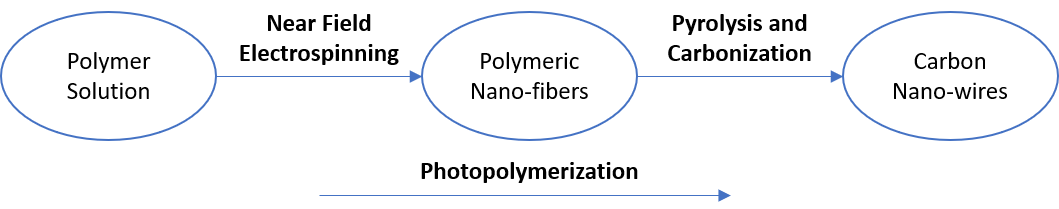
\includegraphics[width=0.95\textwidth]{./Figures/FabricationProcess.png}
\decoRule
\caption[Fabrication Process]{Fabrication process of conductive carbon nano-wires to achieve through the proposed dissertation.}
\label{fig:fabricationFlowChart}
\end{figure}


Nanotechnology has led to the study of different polymer patterning techniques to integrate carbon nano-wires structures. One technique is known as far-field electrospinning, a process in which electrified jets of polymer solution are dispensed to synthesize nano-fibers which are then pyrolyzed at high temperatures. One sub-technique derived from electrospinning is near field electromechanical spinning or EMS. EMS has proved to deliver high control in patterning polymeric nano-fibers. \cite{Cardenas2017}

The proposal is to continue the previous work done in regards to the synthesis of carbon nano-wires. Previous work includes the fabrication of suspended carbon nano-wires by two methods: electro-mechanical spinning and multiple-photon polymerization with a photoresist. \cite{Cardenas2017} This research proposal is intended to focus on electro-mechanical spinning processes only, to bring off polymer solutions that can be electrospun by near field electrospinning (NFES), photopolymerized and pyrolyzed into conducting carbon nano-wires. The polymer solutions described by Cardenas \cite{Cardenas2017} are to be amended to achieve the goal mentioned in the previous statement.

Traditional near-field electrospinning or NFES allows large scale manufacturability combined with spatial control of material deposition. \cite{Madou2011} However, the reported efforts required the use of electric fields in excess of 200 kV/m for continuous operation, resulting in limited control for nano-fiber patterning in traditional NFES processes. Madou et al. \cite{Madou2011} conclude that the current state-of-the-art synthesis processes for polymer nano-fibers lack to yield precise, inexpensive, fast, and continuous manufacturing properties.

%----------------------------------------------------------------------------------------
%	SECTION 1
%----------------------------------------------------------------------------------------



%-----------------------------------
%	SUBSECTION 1
%-----------------------------------


